\chapter{Návrh a architektura NPC systému}

Cílem této kapitoly je ukázat návrh architektury NPC v prostředí Unreal Engine~5, který využívá behaviorální stromy pro jeho řízení. 
Systém byl navržen tak, aby NPC dokázala reagovat na hráče, vnímat objekty v prostředí a v omezené míře spolupracovat s jinými NPC postavami.

V této práci bylo usilováno o dodržení oddělení odpovědností mezi jednotlivými funkčními částmi hry. 
Každá část systému má vymezenou roli: 
postava NPC zajišťuje fyzickou reprezentaci a provádění akcí, AI Controller zpracovává podněty z okolí 
a aktualizuje sdílenou paměť, behaviorální strom na základě těchto dat rozhoduje o aktuálním chování 
a Blackboard slouží jako datové úložiště propojující všechny části.

\section{Přehled systému a jeho komponent}

V projektu jsou vytvořeny dvě konkrétní NPC postavy, \texttt{BP\_Grandpa} a \texttt{BP\_Granny}, které sdílejí společnou rodičovskou třídu \texttt{BP\_NPC}. 
Tato bázová třída obsahuje veškerou herní logiku sdílenou všemi NPC: 
systém animací, správu zbraní, detekci interaktivních objektů v okolí a propojení s globálním stavem levelu. 
Konkrétní odvozené třídy slouží výhradně k odlišení vizuální podoby postav -- jiný skeletální mesh a animační blueprint. 
Přidání dalšího NPC do hry tak nevyžaduje duplikaci AI logiky.

AI logika je sdílena i na vyšší úrovni: obě postavy jsou řízeny stejným AI Controllerem \texttt{IAC\_NPC} a stejným behaviorálním stromem \texttt{BT\_NPC}. Každá instance NPC má přitom vlastní instanci Blackboardu \texttt{BB\_NPC}, takže jejich rozhodování je vzájemně nezávislé i přesto, že vychází ze stejné stromové definice.

Základní komponenty systému jsou:

\begin{itemize}
    \item \texttt{BP\_NPC} -- bázová třída NPC,
    \item \texttt{BP\_Grandpa}, \texttt{BP\_Granny} -- konkrétní NPC postavy,
    \item \texttt{IAC\_NPC} -- AI Controller,
    \item \texttt{BT\_NPC} -- behaviorální strom,
    \item \texttt{BB\_NPC} -- Blackboard,
    \item \texttt{BP\_RoutingManager} -- správce hlídkových tras,
    \item \texttt{BP\_PatrolRoute} -- reprezentace jednotlivé hlídkové trasy.
    \item \texttt{BPC\_InventorySystem} -- Systém inventáře, který využívají jak NPC, tak hráč
    \item \texttt{BPC\_InteractionSystem} -- Systém interakcí, který využívají jak NPC, tak hráč
\end{itemize}

Vzájemné závislosti mezi těmito komponentami jsou znázorněny na obrázku~\ref{fig:components}.

\begin{figure}[htbp]
    \centering
    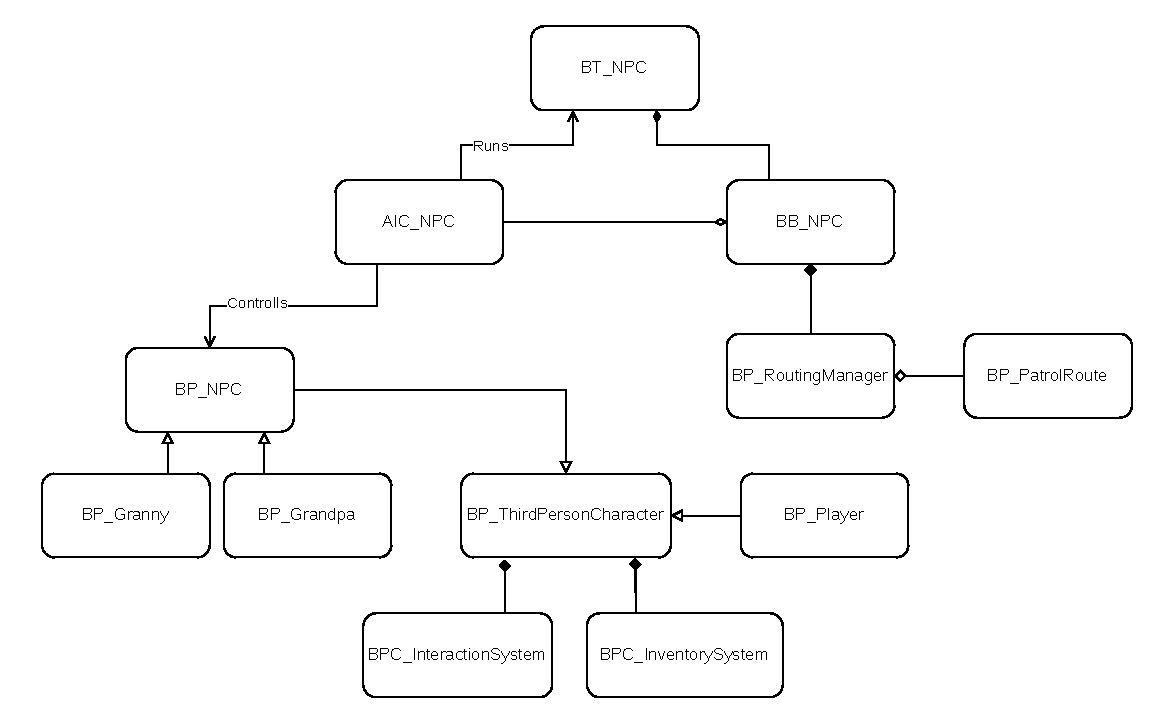
\includegraphics[width=\textwidth]{Figures/components.pdf}
    \caption{Přehled komponent systému NPC a jejich vzájemných vazeb}
    \label{fig:components}
\end{figure}

\section{Rozdělení odpovědností}

Návrh striktně odděluje rozhodování od vykonávání akcí. 
Toto oddělení je klíčovým principem využití behaviorálních stromů: 
strom rozhoduje, co má postava dělat, ale samotné provedení deleguje na třídu NPC.\cite[s.~178]{colledanchise2018}

Třída \texttt{BP\_NPC} implementuje konkrétní akce -- pohyb, útok, manipulaci se zbraní -- a neobsahuje žádnou rozhodovací logiku. 
Reaguje výhradně na příkazy vydané behaviorálním stromem prostřednictvím delegátů a custom eventů. 
Díky tomu lze rozhodovací logiku měnit nezávisle na fyzickém chování postavy.

AI Controller \texttt{IAC\_NPC} plní roli prostředníka mezi herním světem a behaviorálním stromem. 
Zpracovává podněty ze systému percepce, interpretuje je a přepisuje do odpovídajících klíčů Blackboardu. 
Controller sám nerozhoduje o chování NPC -- jeho úlohou je udržovat Blackboard aktuální tak, aby behaviorální strom mohl správně reagovat.

Behaviorální strom \texttt{BT\_NPC} je výhradním místem rozhodovací logiky. 
Na základě hodnot v Blackboardu vybírá odpovídající větev a prostřednictvím Tasků vydává příkazy k provedení konkrétních akcí.

\section{Stavový model NPC}

Chování NPC je strukturováno jako třístavový model. 
Každý stav odpovídá jedné hlavní větvi behaviorálního stromu a určuje, která část stromu bude vyhodnocována:

\begin{itemize}
    \item \textbf{Passive} -- NPC vykonává hlídkovou rutinu, pohybuje se po přidělené trase a příležitostně interaguje s prostředím nebo jinou NPC postavou,
    \item \textbf{Investigating} -- NPC prošetřuje podezřelý podnět, tedy detekovaný zvuk nebo pohyb sledovaného předmětu, na konkrétní souřadnici ve scéně,
    \item \textbf{Attacking} -- NPC reaguje na viděného hráče, vytasí zbraň a zahájí útok.
\end{itemize}

Přechody mezi stavy jsou výhradně v kompetenci AI Controlleru a jsou vyvolány událostmi ze systému percepce. 
Spatření hráče způsobí přechod do stavu \texttt{Attacking}, ztráta hráče ze zorného pole návrat do stavu \texttt{Passive} 
a detekce zvuku přechod do stavu \texttt{Investigating}. 
Aktuální stav je uložen v Blackboardu pod klíčem \texttt{State} jako hodnota výčtového typu \texttt{E\_AIState}. 
Schéma přechodů mezi stavy je znázorněno na obrázku~\ref{fig:state_model}.

\begin{figure}[H]
    \centering
    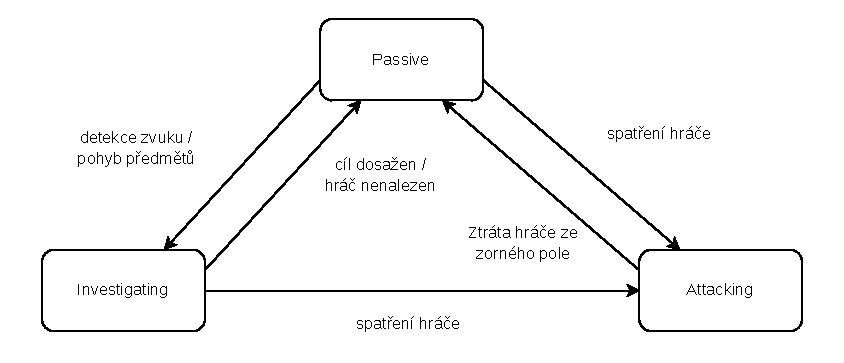
\includegraphics[width=\textwidth]{Figures/state_diagram.pdf}
    \caption{Přehled hlavních stavů NPC a přechodů mezi nimi}
    \label{fig:state_model}
\end{figure}

\section{Architektura behaviorálního stromu}

Behaviorální strom \texttt{BT\_NPC} je sdílen oběma NPC postavami. 
Každá postava spouští svou vlastní instanci stromu s vlastním Blackboardem, takže jejich rozhodování je nezávislé i při použití identické stromové struktury. 
Strom je spuštěn AI Controllerem při převzetí kontroly nad postavou, tedy při události \texttt{OnPossess}.

Na nejvyšší úrovni tvoří strom kořenový \texttt{Selector} se třemi větvemi. 
Každá větev je opatřena dekorátorem, který kontroluje hodnotu klíče \texttt{State} v Blackboardu. 
Selector prochází větve v pořadí od nejvyšší priority:

\begin{enumerate}
    \item \textbf{Attacking} (nejvyšší priorita) -- aktivní, pokud \texttt{State == Attacking},
    \item \textbf{Investigating} -- aktivní, pokud \texttt{State == Investigating},
    \item \textbf{Passive} (výchozí) -- aktivní, pokud \texttt{State == Passive}.
\end{enumerate}

Tato struktura zajišťuje, že útočné chování má vždy přednost před vyšetřováním a hlídkováním, čímž je implementována přirozená hierarchie priorit. 
Celý behaviorální strom je příliš obsáhlý na to, aby jej bylo možné zobrazit zde, a proto jej lze nalézt v příloze této práce~\ref{fig:bt_full}.

\subsection{Větev Passive}

Pasivní větev je nejkomplexnější částí stromu a implementuje hlídkovou rutinu NPC. 
Obsahuje jak Services, které běží periodicky na pozadí, tak Tasks vykonávané sekvenčně:

\begin{itemize}
    \item \texttt{BTS\_EnsurePatrolRoute} (Service) -- periodicky kontroluje, zda má NPC přiřazenou hlídkovou trasu; pokud ne, vyžádá ji od správce tras \texttt{BP\_RoutingManager},
    \item \texttt{BTT\_MakeRouteDecision} (Task) -- rozhoduje na základě aktuálního postupu po trase a náhodné hodnoty, zda NPC změní trasu,
    \item \texttt{BTT\_MoveAlongPatrolRoute} (Task) -- přesouvá NPC na další bod aktuální spline trasy,
    \item \texttt{BTT\_MakeInteractionDecision} (Task) -- rozhoduje, zda NPC interaguje s viděným objektem nebo s jinou NPC postavou; rozhodnutí závisí na typu interakce objektu a náhodné hodnotě \texttt{InteractionChance},
    \item \texttt{BTT\_GoToOtherNPC} (Task) -- naviguje NPC ke druhé NPC postavě,
    \item \texttt{BTT\_InteractWithOtherNPC} (Task) -- provede výměnu informací o pozicích předmětů mezi oběma NPC,
\end{itemize}

\subsection{Větev Attacking}

Útočná větev implementuje reakci na spatřeného hráče. 
Po přechodu do stavu \texttt{Attacking} větev nejprve zkontroluje, zda je zbraň vytasena, a pokud ne, spustí animaci vytasení. 
Poté nastaví AI focus na cíl, přepne NPC do běhu a zahájí útočnou animaci:

\begin{itemize}
    \item \texttt{BTDecorator\_IsWieldWeapon} (Decorator) -- podmínkově spustí vytasení zbraně pouze pokud ještě není vytasena,
    \item \texttt{BTT\_EquipWeapon} (Task) -- přehraje animaci vytasení zbraně,
    \item \texttt{BTT\_FocusTarget} (Task) -- nastaví rotační focus AI na cíl útoku uložený v Blackboardu pod klíčem \texttt{AttackTarget},
    \item \texttt{BTT\_SetMovementSpeed} (Task) -- přepne NPC do běhu nastavením maximální rychlosti pohybu,
    \item \texttt{BTT\_Attack} (Task) -- spustí útočnou animaci; dokončení animace je signalizováno zpět do Tasku prostřednictvím delegátu.
\end{itemize}

\subsection{Větev Investigating}

Vyšetřovací větev je nejjednodušší ze tří. NPC naviguje na souřadnici uloženou v Blackboardu pod klíčem \texttt{PointOfInterest}. 
Po dosažení cílové pozice, nebo pokud cíle nelze dosáhnout, stav automaticky přejde zpět do \texttt{Passive} a NPC pokračuje v hlídkování. 
Tato větev se aktivuje při detekci zvuku nebo při zjištění pohybu sledovaného předmětu.

\section{Tok dat v systému}

Tok informací v systému lze popsat jako sled kroků:

\begin{center}
\texttt{AI Perception} $\rightarrow$ \texttt{AI Controller} $\rightarrow$ \texttt{Blackboard} $\rightarrow$ \texttt{Behavior Tree} $\rightarrow$ akce NPC
\end{center}

AI Controller přijímá podněty ze systému percepce a přepisuje je do Blackboardu: aktualizuje stav NPC, ukládá pozici podezřelého místa nebo referenci na viděný objekt. Behaviorální strom při každém vyhodnocení přečte aktuální hodnoty z Blackboardu, vybere odpovídající větev a prostřednictvím Tasků vydá příkaz ke konkrétní akci. Samotnou akci pak vykoná třída \texttt{BP\_NPC}.

\section{Správa hlídkových tras}

Hlídkové trasy jsou reprezentovány třídou \texttt{BP\_PatrolRoute} jako spline-based křivky rozmístěné ve scéně. 
Pohyb po trase je obousměrný: NPC se pohybuje po bodech spline v jednom směru a po dosažení krajního bodu se otočí a vrátí se zpět po téže trase. 
Pro uzavřené smyčky je index bodu zabalován modulem délky trasy.

Přidělování tras jednotlivým NPC zajišťuje třída \texttt{BP\_RoutingManager}. 
Tento správce řeší problém kolize tras: zamezuje situaci, kdy by dvě NPC hlídkovaly na stejné trase a pohybovaly se synchronně. 
Při vyžádání nové trasy systém iteruje dostupné trasy v náhodně zamíchaném pořadí a přidělí první volnou. 
Obsazenost tras je evidována v interní mapě.

Součástí návrhu jsou tři sady tras odpovídající různým herním fázím (\texttt{Stage 1}, \texttt{Stage 2}, \texttt{Stage 3}). 
Příslušnost tras k dané fázi je určena tagem přiřazeným přímo instancím \texttt{BP\_PatrolRoute} ve scéně. 
Změna herní fáze tak přiřadí NPC jiné trasy bez jakékoliv modifikace behaviorálního stromu.

Variabilita chování je dále zajištěna pravděpodobnostním prvkem: každé NPC má při startu inicializovanou náhodnou hodnotu \texttt{RouteChangeChance} 
v rozsahu $0$--$1$, která určuje pravděpodobnost dobrovolné změny trasy po dosažení určitého úseku. 
Práh pro toto rozhodnutí je po každé změně rovněž randomizován v rozsahu $0{,}25$--$0{,}75$, takže NPC mění trasy nepravidelně a jejich pohyb nepůsobí mechanicky.

\section{Reprezentace znalostí NPC}

Chování NPC v této práci vyžaduje, aby postavy dokázaly pracovat s informacemi o objektech v herním prostředí. 
Nejedná se pouze o okamžitou reakci na podněty, ale také o schopnost zohlednit stav světa při rozhodování.

Znalosti NPC jsou reprezentovány kombinací globálního sdíleného stavu a lokálních dat jednotlivých postav.

\subsection{Globální stav objektů}

Informace o objektech ve scéně jsou spravovány centrálně pomocí třídy \texttt{BP\_GameStateBase}. 
Tato třída obsahuje registr sledovaných objektů, ve kterém jsou uloženy jejich referenční informace.

Každý objekt typu \texttt{BP\_BaseItem} se při inicializaci zaregistruje do tohoto registru a uloží svou výchozí pozici. 
Tato pozice představuje očekávaný stav objektu ve scéně.

Díky tomuto přístupu mají všechny NPC přístup ke konzistentní reprezentaci světa, aniž by bylo nutné 
udržovat redundantní kopie těchto dat pro každou postavu zvlášť.

\subsection{Lokální znalosti NPC}

Každá NPC si zároveň udržuje vlastní seznam známých objektů, který je uložen v její instanci. 
Tento seznam obsahuje reference na objekty, se kterými postava přišla do kontaktu nebo o nich získala informaci.

Lokální seznam slouží k:
\begin{itemize}
    \item uchování informací relevantních pro konkrétní NPC,
    \item vyhodnocování interakcí s objekty,
    \item rozhodování v rámci behaviorálního stromu.
\end{itemize}

Tato data nejsou sdílena přímo mezi NPC, ale každá postava je interpretuje samostatně na základě 
globálního stavu a vlastních zkušeností.

\subsection{Inicializace znalostí}

Při spuštění hry dojde k inicializaci registru objektů a jejich základních vlastností. 
NPC následně pracují s těmito daty během svého běžného chování, zejména v rámci pasivní větve behaviorálního stromu.

\subsection{Detekce změn v prostředí}

Změna stavu objektu je určena porovnáním jeho aktuální pozice s referenční hodnotou uloženou v globálním registru.

Pokud se tyto hodnoty liší, je objekt považován za přesunutý nebo chybějící. 
Tato informace je následně využita při rozhodování NPC, například pro přechod do stavu \textit{Investigating}.

Tímto způsobem je možné detekovat změny ve světě bez nutnosti složitějších mechanismů sledování historie.

\section{Komunikace mezi NPC}

Komunikace mezi NPC je realizována prostřednictvím Tasku \texttt{BTT\_InteractWithOtherNPC}, který se spouští v rámci pasivní větve behaviorálního stromu, když se dvě NPC dostatečně přiblíží. 
Mechanismus výměny informací probíhá ve třech krocích.

Nejprve aktivní NPC zjistí z globálního herního registru, tedy z \texttt{BP\_GameStateBase}, jaká je domácí neboli referenční pozice 
sledovaného předmětu -- tedy kde by měl předmět být. 
Poté přečte ze záznamu paměti druhé NPC, kde tento předmět druhá NPC naposledy viděla. 
Nakonec obě hodnoty porovná.

Pokud jsou pozice shodné, předmět nebyl přemístěn a NPC pokračují v hlídce. 
Pokud se pozice liší, byl předmět přemístěn hráčem. 
V takovém případě jsou u obou NPC nastaveny Blackboard klíče \texttt{LostItem?} na hodnotu \texttt{true} a \texttt{SearchShed} na hodnotu \texttt{true}, čímž jsou 
obě postavy instruovány k prohledání určitého místa. Zápis do Blackboardu druhého NPC probíhá přímým přístupem přes jeho AI Controller, bez použití centrálního 
koordinátora.

Jedná se o decentralizovaný mechanismus spolupráce: každé NPC si informace aktivně zjišťuje při každém setkání s partnerem 
a v případě nesouladu koordinovaně zahájí vyšetřování. 
Tím je naplněn požadavek na implementaci spolupráce mezi NPC postavami.

\section{Reakce na hráče a prostředí}

Reakce NPC na hráče je řízena systémem AI Perception implementovaným v AI Controlleru. 
Systém percepce pracuje se dvěma smysly: zrakem (\texttt{AISense\_Sight}) a sluchem (\texttt{AISense\_Hearing}).

Při zpracování vizuálních podnětů rozlišuje Controller tři scénáře. 
Pokud NPC spatří hráče, okamžitě přejde do stavu \texttt{Attacking} -- behaviorální strom při dalším vyhodnocení aktivuje útočnou větev s nejvyšší prioritou. 
Pokud hráč opustí zorné pole, NPC se vrátí do stavu \texttt{Passive}. 
Pokud NPC zaznamená interaktivní objekt ve scéně, uloží referenci na něj do Blackboardu pod klíč \texttt{SeenInteractible}, který pasivní větev stromu využije 
při rozhodování o interakci.

Zvukové podněty zpracovává Controller odděleně: pokud NPC uslyší zvuk a aktuálně není ve stavu \texttt{Attacking}, přejde do stavu \texttt{Investigating} 
s cílovou souřadnicí zdroje zvuku. 
Pokud NPC již útočí, zvuk je ignorován -- útok má vyšší prioritu a přechod do vyšetřovacího stavu by ho nežádoucně přerušil.

\section{Návrhová rozhodnutí}

Při návrhu systému byla přijata následující klíčová rozhodnutí:

\begin{itemize}
    \item \textbf{Společná bázová třída NPC} -- odděluje vizuální identitu od AI logiky a umožňuje přidávání nových typů NPC bez duplikace kódu. 
    Nová postava vyžaduje pouze nový mesh a animační blueprint.

    \item \textbf{Sdílený behaviorální strom s nezávislými Blackboardy} -- obě NPC sdílejí jednu definici stromu, ale každá rozhoduje na základě vlastních dat. 
    Tím je zajištěna konzistence chování při minimálním počtu assetů.

    \item \textbf{Oddělení rozhodování od vykonávání} -- AI Controller a behaviorální strom rozhodují, třída NPC vykonává. 
    Toto oddělení odpovídá doporučenému architektonickému vzoru pro využití behaviorálních stromů v Unreal Engine~5.

    \item \textbf{Blackboard jako centrální sdílená paměť} -- propojuje Controller, strom a Tasky bez přímých závislostí mezi nimi; každá část systému čte a zapisuje pouze do Blackboardu.

    \item \textbf{Pravděpodobnostní inicializace chování} -- náhodná inicializace hodnot \texttt{RouteChangeChance} a \texttt{InteractionChance} při startu 
    každého NPC zajišťuje, že i při sdíleném stromu se obě postavy chovají mírně odlišně a jejich pohyb nepůsobí synchronně.

    \item \textbf{Správce tras bez kolizí} -- \texttt{BP\_RoutingManager} zamezuje obsazení stejné trasy dvěma NPC současně, čímž zvyšuje přirozenost hlídkování 
    a zabraňuje vizuálně rušivé synchronizaci pohybu.
\end{itemize}

